\documentclass[conference]{IEEEtran}
\IEEEoverridecommandlockouts
% The preceding line is only needed to identify funding in the first footnote. If that is unneeded, please comment it out.
\usepackage{cite}
\usepackage{amsmath,amssymb,amsfonts}
\usepackage{algorithmic}
\usepackage{graphicx}
\usepackage{textcomp}
\usepackage{subfigure}
\usepackage{caption}
\usepackage{graphicx} %use graph format
\usepackage{epstopdf}

\def\BibTeX{{\rm B\kern-.05em{\sc i\kern-.025em b}\kern-.08em
    T\kern-.1667em\lower.7ex\hbox{E}\kern-.125emX}}

\newcommand{\tabincell}[2]{\begin{tabular}{@{}#1@{}}#2\end{tabular}}
    
\begin{document}

\title{A Hybrid Model based on Multi-Dimensional Features for Insider Threat Detection\\
\thanks{Identify applicable funding agency here. If none, delete this.}
}

\author{\IEEEauthorblockN{1\textsuperscript{st} Given Name Surname}
\IEEEauthorblockA{\textit{dept. name of organization (of Aff.)} \\
\textit{name of organization (of Aff.)}\\
City, Country \\
email address}
\and
\IEEEauthorblockN{2\textsuperscript{nd} Given Name Surname}
\IEEEauthorblockA{\textit{dept. name of organization (of Aff.)} \\
\textit{name of organization (of Aff.)}\\
City, Country \\
email address}

}

\maketitle

\begin{abstract}
Insider threats have shown their power by hugely affecting national security, financial stability, and the privacy of many thousands of people.
A number of techniques have been proposed to detect insider threats either by comparing behaviors among different individuals or by comparing the behaviors across different time periods of the same individual. However, due to the  fact that the behaviors of insider threats are always complex and diverse, both of them always fail to identify certain kinds of inside threats.
This paper focuses on proposing a hybrid model to detect insider threats  based on multi-dimensional features.
First, based on the isolation Forest algorithm,  
an Across-Domain Anomaly Detection(ADAD) model is proposed to dentify anomalous behaviors that deviates from the behaviors of their peers by using multi-source information. Second, we propose an Across-Time Anomaly Detection(ATAD) model to measure the degree of unusual changes of a user's behavior  by implementing an improved Markov model. Finally, our proposed hybrid model present a fusion
method to integrate the evidences from the above two models. With the data lasting 17 months, we evaluate our proposed models comprehensively. The results demonstrate the robust performance of the ADAD and ATAD models and the hybrid model is demonstrated to outperform the two separate models obviously.


\end{abstract}

\begin{IEEEkeywords}
insider threat detection, information fusion, hybrid model, Isolation Forest, Markov Model
\end{IEEEkeywords}

\section{Introduction}

Insider threats are threats with malicious intent directed towards organizations by people internal to the organization\cite{b1}.
These include physical sabotage activities, theft of confidential data and business secrets, and fraud. Financial loss and reputation damage caused by this ``known unknow'' cybersecurity threat far outweighs that caused by external attacks. One of the most recent articles from CSO magazine\cite{b3} compared the cost between external and internal attacks and noted that while it takes about 50 days to fix a data breach caused by an internal attack, it only takes 2 to 5 days in the case of external attacks. Nowadays, researchers have proposed different models to prevent or detect the presence of attacks.

Existing literature focuses on two types of insider threat detection 
models: data driven detection models \cite{b4}\cite{b5} and behavior driven detection models\cite{b2}\cite{b6}: 

\noindent \emph{1)} The first model aims to find a normal portrait in all users data in order to detect insider threat that deviates from  this normal portrait by comparing with their peers\cite{b10}. Figure 1 shows an example of insider threats which can be detected by this kind of model \cite{b10}. After getting off work, the general behavior is going home to have a rest. By contrast, few of users secretly deal with the company's confidential documents in the workplace when others are sunk in sleep at midnight, and are more likely to be a insider threat. However, merely comparing the behaviors among peers,  this kind of models fails to detect a malicious insider who tries to behave like a normal user to cover up his evil.

\noindent \emph{2)} The second model regards the abnormal changes in the behavior as the basis for inside threat detection by comparing behaviors of themselves in different time periods.
Figure 1 also show an example to depict a malicious insiders detection based on the behavior-driven method\cite{b8}. Over a long period in the past, the regular behavior of the user was to click on the browser after booting, view the email, and then reply. But one day, he acted abnormally: he connected the mobile device after booting, and had a series of operations on the file-copy to steal the company's confidential documents. These abnormal behaviors don't match his usual styles of doing things. It is worth to note that although the malicious insider may try to behave like a normal user, the threat can also be detected based on the deviation from his regular behavior routines.
However, the model is unable to recognise situations where a user systematically attacks an
organisation over a long-term period. \cite{b2}. 

Thus, Insider threat surveys\cite{b9} suggest the problem of insider threat detection cannot be defined only as a data or behavior driven problem. Therefore, it is necessary to model the problem as data and behavior driven problems, based on which a effective model needs to be proposed.

Thus, based on multidimensional features, this paper proposes a hybrid model that combines a data driven model with a behavior driven model to detect insider threat in a more robust and accurate manner.
First, the multi-dimensional features extracted from data collected  from an enterprise network is formatted and fed separately into the two separate models. Second, each model generates an abnormal score to represent the degree of users' unusual behaviors. Finally, the abnormal scores of two models are fused to be the final abnormal score of each user, and a user is identified to be a insider threater if the anomaly score exceeds the threshold. 
After a wide range experiments, it is 
verified that the hybrid model can detect insider threats in a more robust and accurate manner.
Overall, the contributions of this paper can be summarized as follows:


\begin{enumerate}
\item 
We apply the isolation Forest to detect behavioral inconsistencies among the behaviors of users. In this model, we extract and combine temporal features from multi-source data comprehensively when constructing the user's portrait.

\item We propose an improved model based on Markov to identify users' unusual changes. The proposed model considers all historical behaviors of users as the contextual information. As compared with the existing predictor of Markov model \cite{b10}, our proposed approach show higher efficiency.

\iffalse
\item We propose a hybrid model for accuracy detection of insider threats by fusion methods which is able to determine malicious insiders that not only act inconsistent with peers but also have unusual change compared with their historic behavior and  achieve the accuracy of 95\%. 
\fi
\item We propose a hybrid model based on multi-dimensional features for insider threat detection. The model is able to determine malicious insiders that not only act inconsistent with their peers but also have unusual changes compared with their historic behaviors. 
Through extensive experiments, we abtain the accuracy of 95\% through the proposed model, which is of great significance in industry and scientific research.
 


\end{enumerate}

The remainder of this article is structured as follows. 
section 2 presents the related work about the research.
Then, section 3 details our approach. Next, in section 4, 
we detail our implementation of the models and analyze the experiments reaults. 
Finally we conclude in section 5, also presenting limitation of our work.

\begin{figure*}[htb]
\centerline{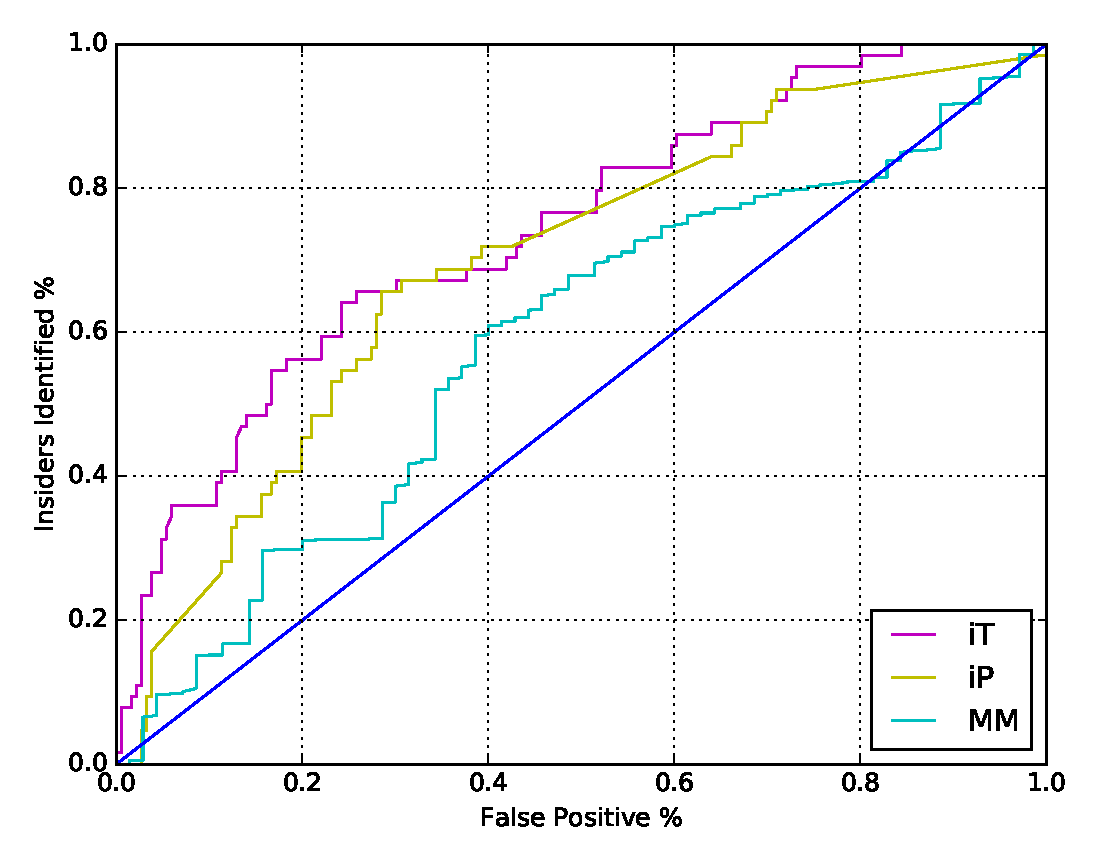
\includegraphics[width = 0.8\textwidth]{figure/figure1.eps}}
\caption{Example of insider threat.}
\label{fig}
\end{figure*}


\section{Related work}
%在增加一部分related work:hybrid model 或者多特征融合
The topic of insider threat has recently received much attention in the literature. Researchers have proposed different models aimed at preventing or detecting the presence of attacks \cite{b11}\cite{b12}. To elicit the state of art, the work
presented here is focused on the approaches of detecting  insider threat based on data-driven methods and behavior-driven methods.

With regard to the data-driven methods, Mathew et al.\cite{b13} detected inside threat on account of user access patterns, Eberle et al. \cite{b14} used social graphs to detect the abnormal. More recently, Eldardiry et al. \cite{b15} have also proposed a system in managing insider
attacks which compared user’s behaviour based on peer baselines.
Michael Goldsmith applied a layered architecture by  fusing across multiple levels information to detect anomalies from heterogeneous data\cite{b16}. Hoda et al. \cite{b13} detect peer groups of users and modeling user behavior with respect to these peer groups, and subsequently detect insider activity by identifying users who deviate from their peers with respect to the user behavior models. 
There have also been various approaches based on data-driven to detect abnormal\cite{b7}\cite{b8}. 
However, they did not factor in the changes of user behaviors over time. We note that while a common activity not be suspicious, a rare change of the order  common activity can be. So some methods based on behavior-driven are proposed to solve the problems. 

There are several literatures based on behavior-driven models\cite{b10}\cite{b11}\cite{b12}. 
Tabish Rashid \cite{b37} takes the change of user behavior  over time to detect the anomaly and achieved some results. However, these behavior-driven models just work out based on unusual change of user behavior, but will miss recognising situations where a user systematically attacks an organisation over an extended time-framework.

\iffalse
Considering these two factors, we propose 
a hybrid model based on multi-dimensional features for accuracy detection of anomalies.
We fusion two method based on data and behavior.
The first one, we compare behaviours across different individuals, while in the latter, we compare behaviours acorss different times for the same individual.  
We abtain the accuracy of 95\% through the proposed model, which is of great significance in industry and scientific research.
\fi




\section{Overview of proposed approach}
\iffalse
We propose a fusion method based on multi-dimensional features for insider threat detection which is illustrated in Figure2. First, for multi-source information,we extract features in two dimensions,one we count and analyze the characteristics of each domain(e.g., logons),and the other we focus on time-series behaviors of user to identify changes in activities of a user compared to that user’s past activities.

After the features extraction, the architecture has two main components - one component for detecting abnormality across information sources (or domains)through Iforest algorithm named “Across-Domain Anomaly Detection(ADAD)”, and another for detecting inconsistencies across time named “Across-Time Anomaly Detection(ATAD)” - which are then fused together to improve accuracy and robustness. These components are briefly described in next section.
\fi

We propose a hybrid model based on multi-dimensional features for insider threat detection which is illustrated in Figure2. First, we analyze the characteristics of each domain(e.g., logons) from multi-source information as parameters into “Across-Domain Anomaly Detection(ADAD)” to get anomaly scores. Second, we extract the features of time-series behaviors of users from multi-source information, then we identify changes in activities of a user compared to that user’s past activities through “Across-Time Anomaly Detection(ATAD)” to get anomaly scores. Finally, we combine the anomaly scores from the two components to detect insider threat. Next, we will introduce the experimental data. 


\begin{figure}[htb]
\centerline{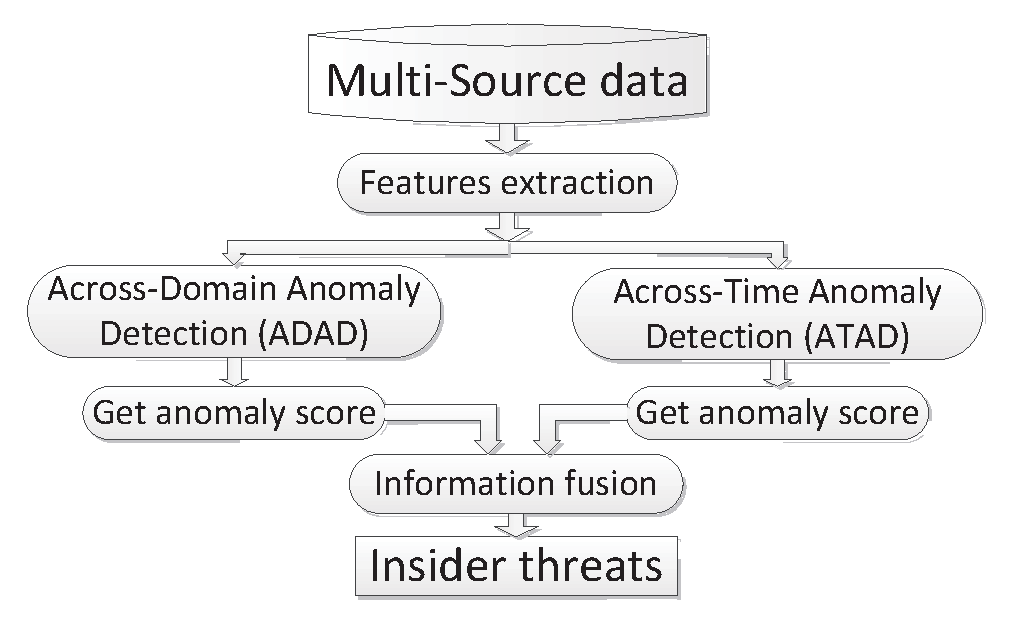
\includegraphics[width = 0.35\textwidth]{figure/figure2.eps}}
\caption{Anomaly Detection Framework.}
\label{fig}
\end{figure}

\subsection{The Data Set}

Due to the lack of availability of proper insider threat datasets, we have utilized the insider threat
dataset published by CERT Carnegie Mellon University for this research \cite{b39}. The dataset “R4.2.tar.bz” has been used for this analysis. According to the dataset owners, this is a “dense needle” dataset with a fair amount of red team scenarios. This dataset consists of six broad types of data records (HTTP, logon, device, file, email and psychometric) of 1000 employees over a 17 months period. 
All HTTP records contain user, PC, URL and web page content with time stamps. “Logon.csv” consists of user logon/logoff activities with the corresponding PC with timestamps. “Logon” activity corresponds to either a user login event or a screen unlock event, while the “Logoff” event corresponds to user logoff event.  The third data file “device.csv” is a collection of data records of removable media usage. It indicates insert/remove actions with the relevant user, PC, and timestamp. Details of file copies are stored in “file.csv” file with date, user, PC, filename, and content.
We should note that the CERT Dataset contains the ground truth for each user (when they are acting maliciously or not), which allows us to monitor the success or failure of our experiment.

\section{KEY METHODOLOGIES}
In this section, we describe our across-domain anomaly detection(ADAD) model in detail at first. We next describe our proposed improved MM based on across-time to detect insider threats. Finally, we introduce the fusion method combining ADAD and ATAD.


\subsection{Approach 1:Across-Domain Anomaly Detection(ADAD)}\label{AA}

This framework will utilize multidimensional inputs, such as user interactions with hardware
assets, logon records and operation on file, to identify anormal users, who behave differently from their peers.
\iffalse
For example, most people would sleep at midnight, but few maybe login the system and do some business such as copying lots of files. This behavior different from most peers not only occur in a domain, but all domains. 
So  
We believe that it is sufficient to consider all behaviors from every domain to characterize the user's behavior. 
\fi
The figure 2 reports the structure of the approach.


\begin{figure}[htb]
\centerline{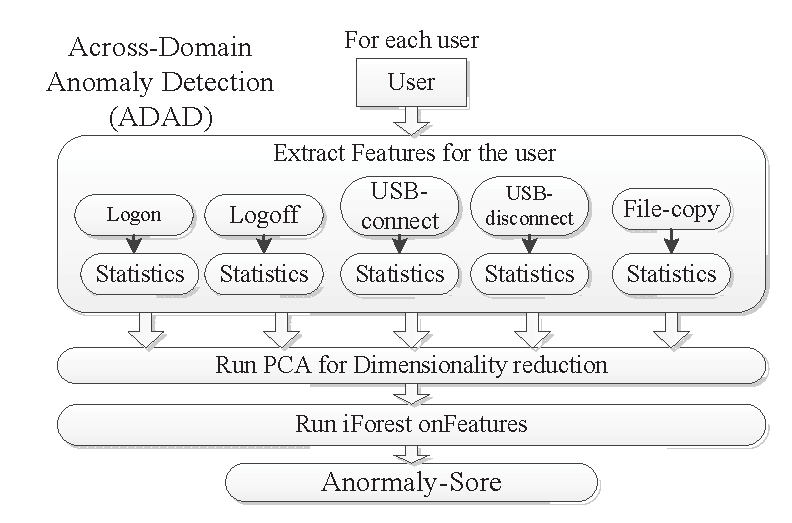
\includegraphics[width = 0.35\textwidth]{figure/figure3.eps}}
\caption{An overview of the Across-Domain Anomaly Detection(ADAD).}
\label{fig}
\end{figure}

\subsubsection{Feature Extraction}


\textbf{Individual Logon-Logoff Behaviors.} This parameters can be used in identifying users abnormal logon/logoff activities, as most disgruntled insiders tend to commit malicious activities after hours \cite{b40}. Identifying users’ baseline behavior on system/device access is an essential part of malicious insider threat detection problem. For normal users and abnormal users, two parameters ( the average of their maximum and mode) logon and logoff values have been calculated for every hour shown as Figure4. 
%width=2.8in


\begin{figure*}[!t]
\centering
\subfigure[Logon behavior]{
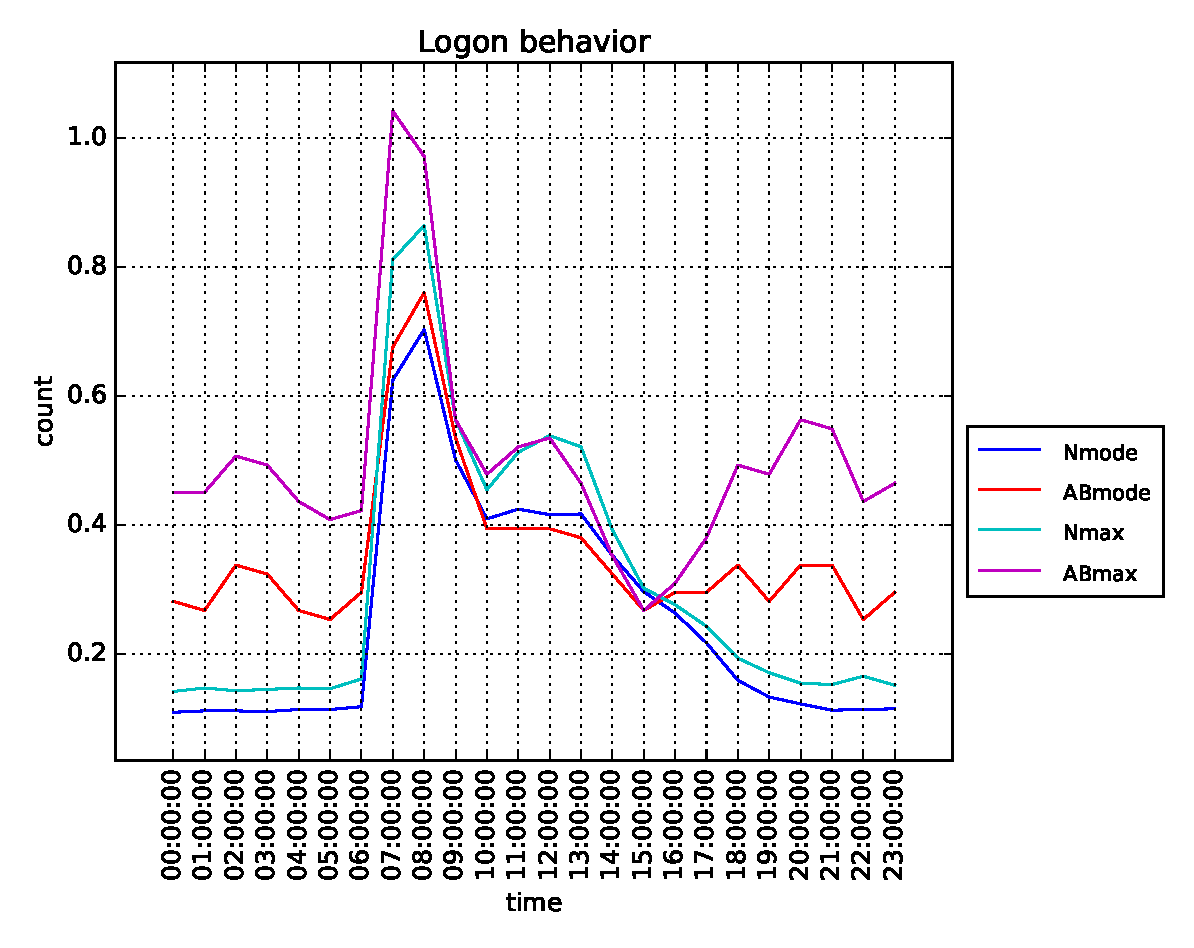
\includegraphics[width=0.18\textwidth]{figure/figure41.eps}
} 
\subfigure[Logoff behavior]
{
 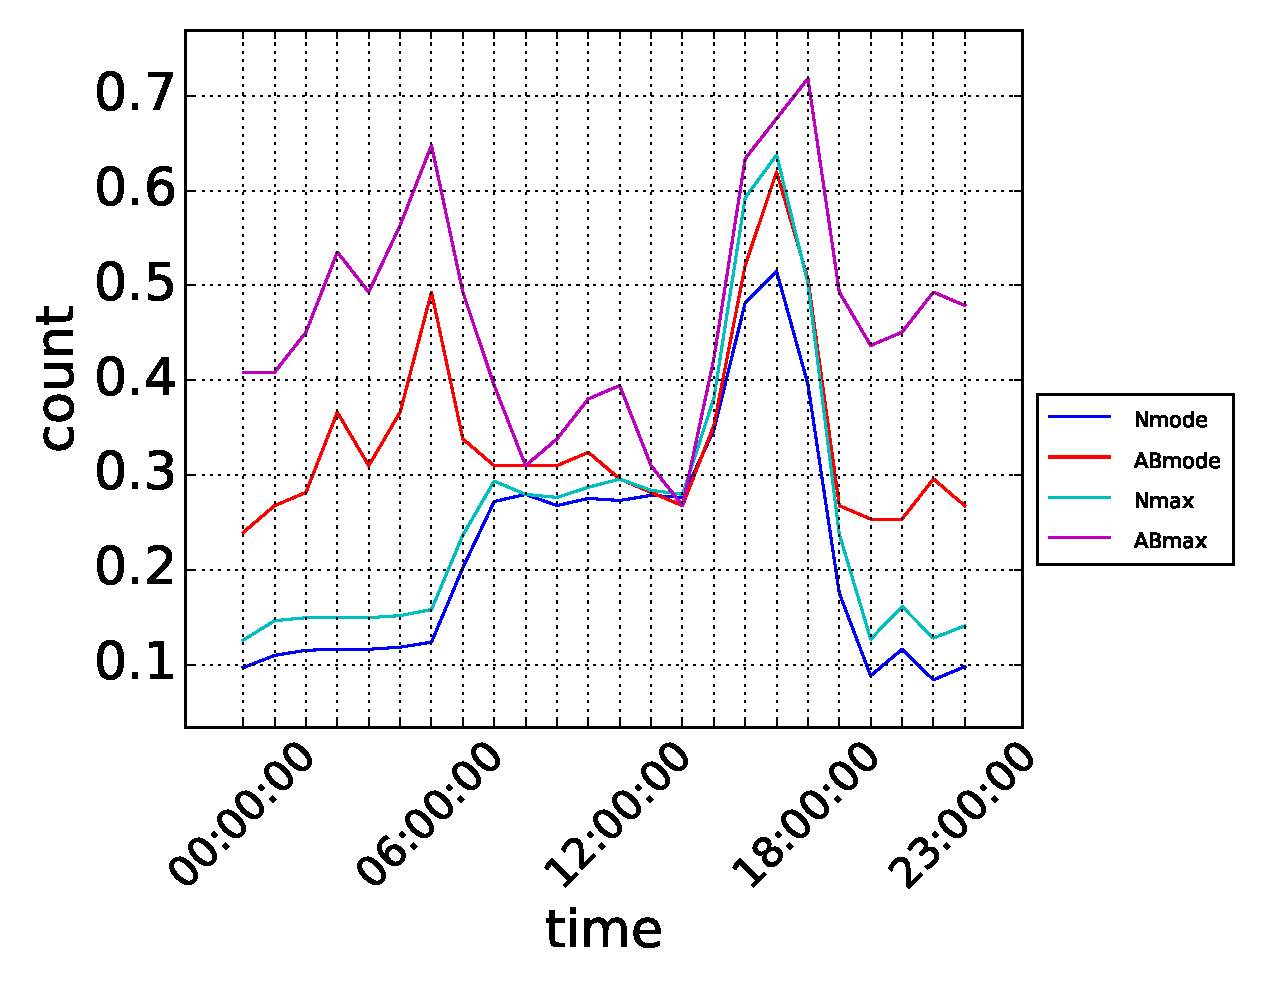
\includegraphics[width=0.18\textwidth]{figure/figure42.eps}
}
%\caption{ Users’ logon and logoff behavior }
\subfigure[USB connect]{
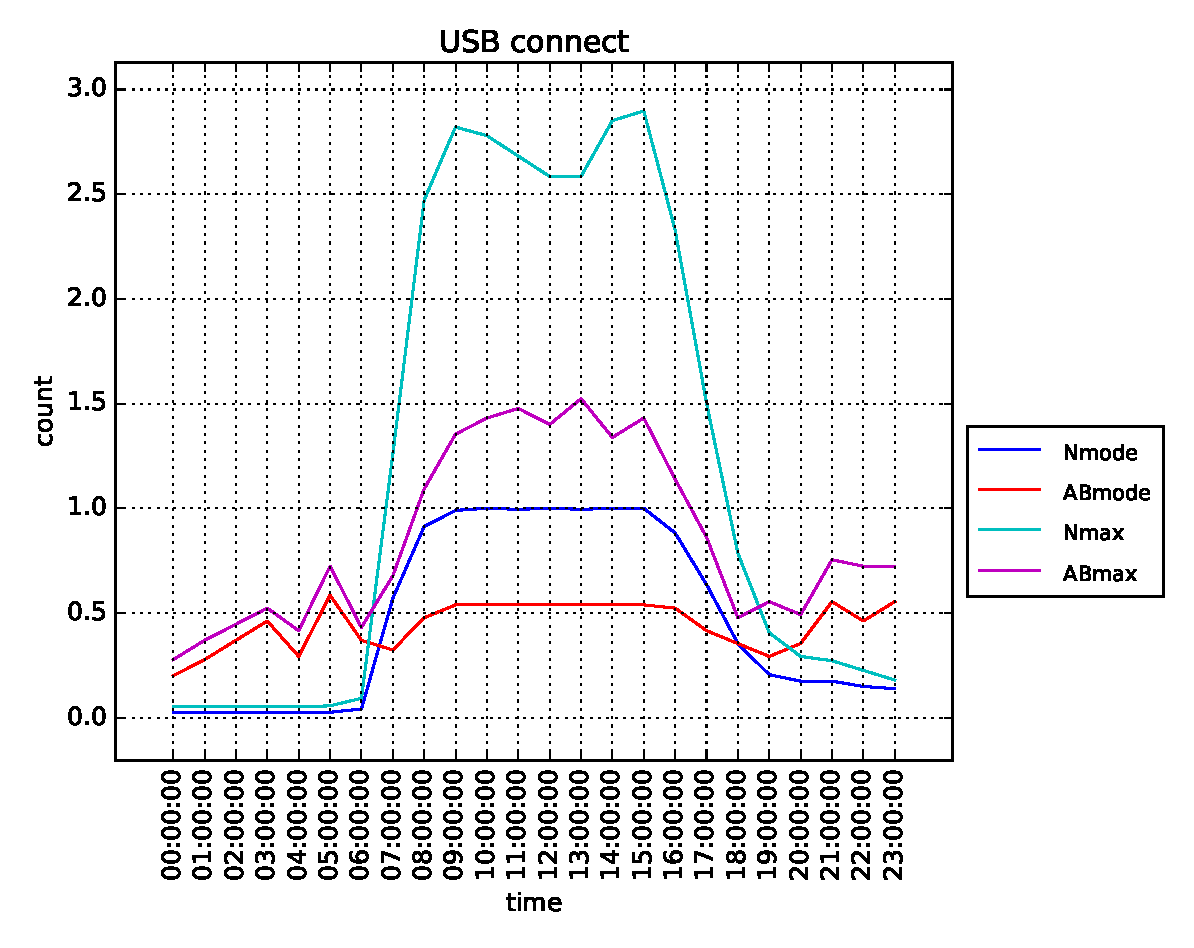
\includegraphics[width=0.18\textwidth]{figure/figure51.eps}
} 
\subfigure[USB disconnect]
{
 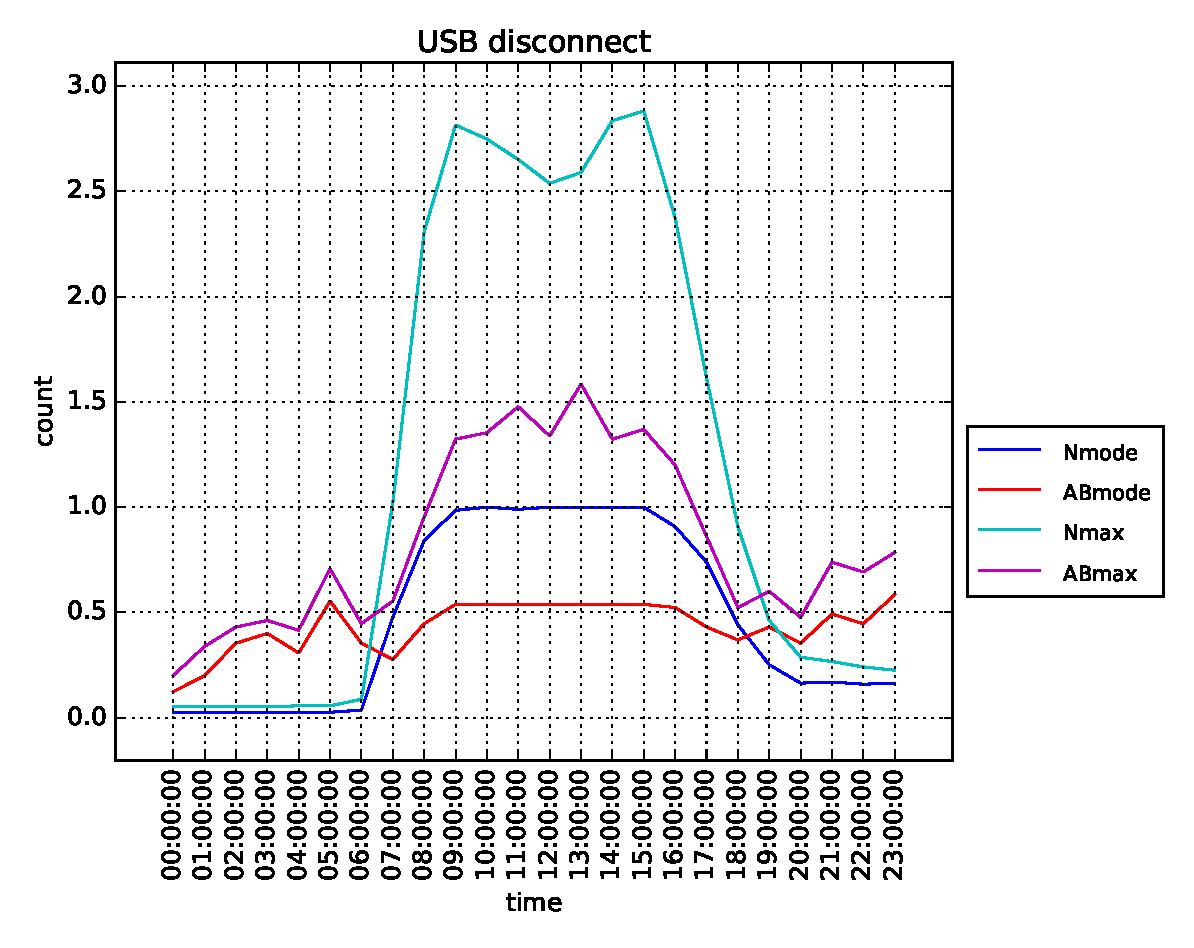
\includegraphics[width=0.18\textwidth]{figure/figure52.eps}
}
\subfigure[File copy]
{
 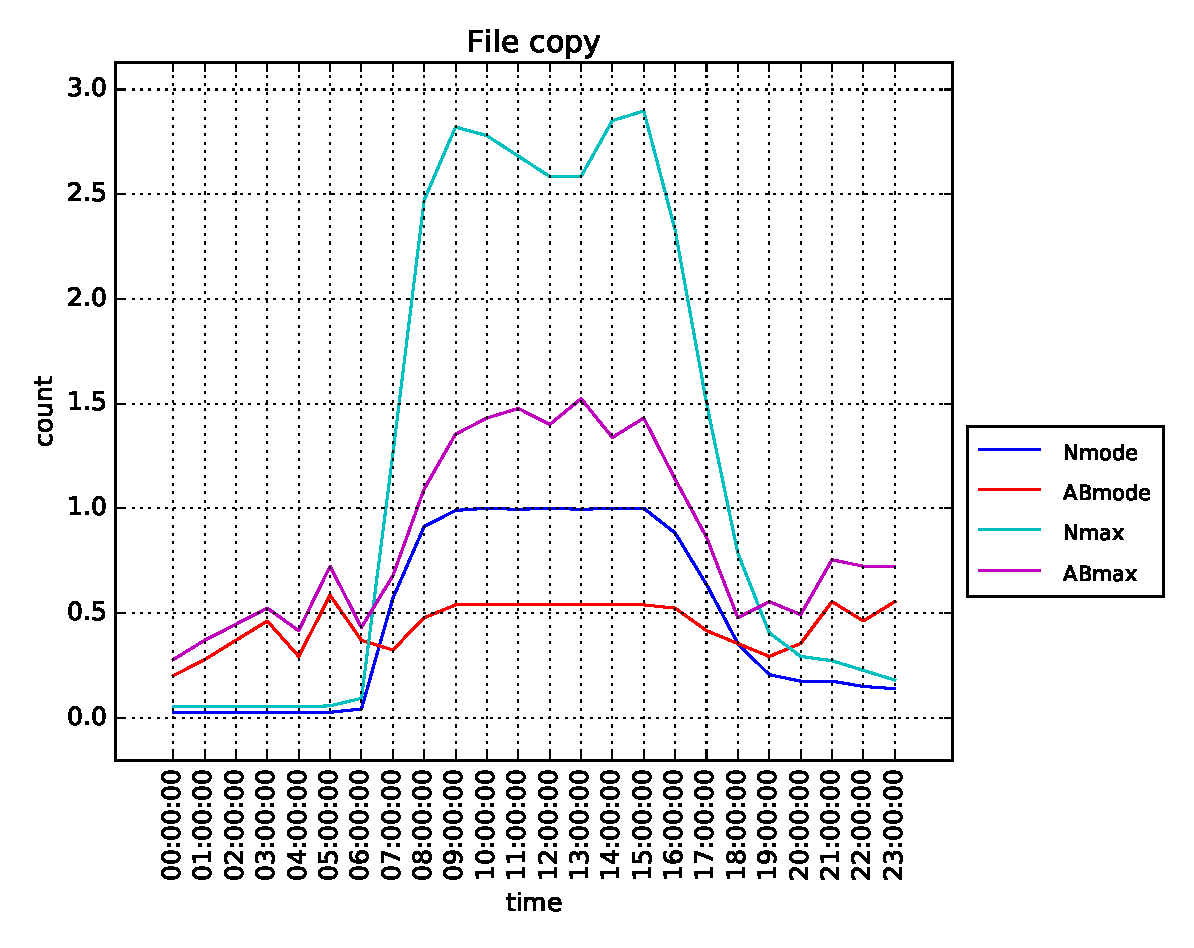
\includegraphics[width=0.18\textwidth]{figure/figure53.eps}
}
\caption{ Removable media usage behavior }
\label{fig5}
\end{figure*}

\textbf{Removable media usage.}
Removable media is among the most popular method used in theft of Intellectual Property (IP) in extracting confidential information from organizations \cite{b41}. Tracking the use of removable media can be an excellent information source for identifying suspicious events by trusted insiders . Baseline behavior of removable media usage is captured by the average of their maximum and mode time of “Insert” and “Remove” activities as in the logon/logoff event analysis. Figure4 shows it.

\textbf{File copy Behaviors.}
The behaviors of file copying has some differences bwtween normal users and abnormal users.
The average of the number of files copied per hour by normal and abnormal is shown in the figure4. 

From the figure4, we found that there is a a big difference in behavior between normal user and abnormal user at different times, so we decide to merge the times of behavior every 6 hours as the parameter to input to our ADAD model. Figure 5 is an illustration of the parameters.

\iffalse
\textbf{Individual Logon-Logoff Behavior.} Figure 4(a) is an illustration of users logon behavior for the
entire period of the dataset. By looking at this graph, it is evident that the majority of logon activities occur during early office hours, which can be interpreted as the first logon event of the day. This phenomenon applies to everyone.  The logon times which we need to pay more attention are the events which happen during after office hours. We can identify abnormal users who have maximum logon times occurred during the late night, which indeed is unusual for normal operations. One of the other critical parameters of insider threat detection, the “logoff” behavior of users are illustrated in Figure 4(b). This graph also shows the mode and maximum logoff times of each user for the entire period. As can be seen on the graph majority of “logoff” events happen during late office hours for normal users. For abnormal users, the times increased significantly of logoff behavior. they are more active during after office hours.

\textbf{Removable media usage.} Figure 5 is an illustration of users’ removable media usage statistics.
Similar to logon/logoff analysis, time dependencies of removable media usage has also been investigated. Figure 5(a) and (b) shows the maximum and mode times for USB connect and disconnect events respectively. We can find that the maximum of times for USB connect and disconnect events of the normal user are generally higher than the abnormal user, which can be understood as the need of some jobs. But the times of the behavior frequently occurrences in the morning 0:00 and 6:00, in which  there almost no operation for the normal user.  Abnormal users have a greater probability of abnormal behavior during the period, for example, copy the company internal documents.
Figure 5(c) demonstrate the variation of users daily number of file accesses. To identify suspicious file copies we have considered the maximum and mode of the number of file copies per day by an individual. From the illustration, the normal are more inclined to carry out the operation of the file in the middle of the night compared with the normal.


In summary, we found that there is a a big difference in behavior between normal user and abnormal user at different times, so we decide to merge the times of behavior every 6 hours as the parameter to input to our ADAD model. Figure 5 is an illustration of the parameters.



\begin{table}[tbp]
\caption{Selected parameter set.}
\centering  % 表居中
\begin{tabular}{lc}  % {lccc} 表示各列元素对齐方式,left-l,right-r,center-c
\hline
Module	&Parameter\\ \hline
	
Logon events	& \tabincell{c}{Maximum/Mode Alogon counts(00:00-06:00)\\Maximum/Mode Blogon counts(06:00-12:00)\\Maximum/Mode Clogon counts(12:00-18:00)\\Maximum/Mode Dlogon counts(18:00-24:00)}\\\hline

Logoff events	& \tabincell{c}{Maximum/Mode Alogoff counts(00:00-06:00)\\Maximum/Mode Blogoff counts(06:00-12:00)\\Maximum/Mode Clogoff counts(12:00-18:00)\\Maximum/Mode Dlogoff counts(18:00-24:00)}\\\hline

Removable Media	& \tabincell{c}{Maximum/Mode Aconnect counts(00:00-06:00)\\Maximum/Mode Bconnect counts(06:00-12:00)\\Maximum/Mode Cconnect counts(12:00-18:00)\\Maximum/Mode Dconnect counts(18:00-24:00)\\Maximum/Mode Adisconnect counts(00:00-06:00)\\Maximum/Mode Bdisconnect counts(06:00-12:00)\\Maximum/Mode Cdisconnect counts(12:00-18:00)\\Maximum/Mode Ddisconnect counts(18:00-24:00)}\\\hline

File copy events	& \tabincell{c}{Maximum/Mode Afilecopy counts(00:00-06:00)\\Maximum/Mode Bfilecopy counts(06:00-12:00)\\Maximum/Mode Cfilecopy counts(12:00-18:00)\\Maximum/Mode Dfilecopy counts(18:00-24:00)}\\\hline

\end{tabular}

\end{table}

\fi


\begin{table}[tbp]
\caption{Selected parameter set.}
\centering  % 表居中
\begin{tabular}{ll}  % {lccc} 表示各列元素对齐方式,left-l,right-r,center-c
\hline
Module	&\tabincell{c}{Parameter\\
					(00:00-06:00)(06:00-12:00)\\
					(12:00-18:00)(18:00-24:00
					}\\ \hline
	
Logon events	&Maximum/Mode Logon counts\\\hline

Logoff events	&Maximum/Mode Logoff counts \\\hline

Removable Media	&\tabincell{c}{Maximum/Mode Connect  counts\\Maximum/Mode Disconnect counts}\\\hline

File copy events	& Maximum/Mode Filecopy counts\\\hline

\end{tabular}

\end{table}

After the experiment we found that the features we extracted had noise effects (which in detail in the experimental part), in order to achieve higher accuracy, we use PCA\cite{b42} for denoising. All feature columns are normalized before the PCA decomposition is performed. By default, we consider a decomposition of the features to a 2-D space.

\subsubsection{Anomaly Detection}

Due to the complex nature of insider threat problem, it is extremely hard to pinpoint a user as a malicious insider. Therefore, the first step should be the identification of possible malicious insiders who are maximally deviating from peers as well as their normal behavior. Therefore, as the second stage of our analysis, we will focus on implementing an anomaly detection algorithm based on the the  properties identified at the previous stage of this analysis. The anomaly detection algorithm adopted in this analysis is the ''Isolation forest`` algorithm, which stands out in effectively separating anomalous events from the rest of the instances \cite{b43}.
\iffalse
Isolation forest Algorithm - iForest: The isolation forest algorithm is a model-based approach which
explicitly isolates anomalies without constructing a typical profile instance. Linear time complexity with a low constant and low memory requirements drives us to use it in our experiments as the enormous amount of information need to be analyzed in the field of insider threat. The use of the isolation forest algorithm for this work is part of the overall research effort within our research group at RMIT University and CA Pacific, with the details as presented in \cite{b44}, where it is applied to a very large enterprise system for anomaly detection. This algorithm also performs well with a large number of irrelevant attributes and instances where training data set does not contain any anomalies. This method generates an ensemble of iTrees for a given dataset and the instances with the short average path of iTrees are considered to be anomalies. If the calculated anomaly score value, s is very close to 1 it can be regarded as a definite anomaly. Instances with s much smaller than 0.5 can be considered normal situations. If all the instances return s ≈ (0.5), then the entire sample deemed to be not having any distinct anomalies.
\fi

\subsection{Approach 2: Across-Time Anomaly Detection(ATAD)}

Markov Model (MM)\cite{b45} is an extremely powerful
tool to model temporal sequence information. It has been
widely used in temporal pattern recognition problems (e.g.,
speech recognition, bioinformatics, gesture recognition) due
to its high detection rate \cite{b55}. MM has also been used
in the general area of intrusion detection by some notable
works (\cite{b54}). Since we model users behaviors as a
temporal sequence of observable query anomaly scores in
our work in this section, and proposed an improved MM model to detect insider threats.
\iffalse  
In this section we use Markov chain model \cite{b45} to detects the insider threat who tries to behave like a normal user to cover up his evil by comparing
behaviors of themselves in different time periods.
\fi
Figure 6 shows a graphical overview of the processing approach and pipeline we use, and the remainder of this section is dedicated to describing each stage in it.
\begin{figure}[htb]
\centerline{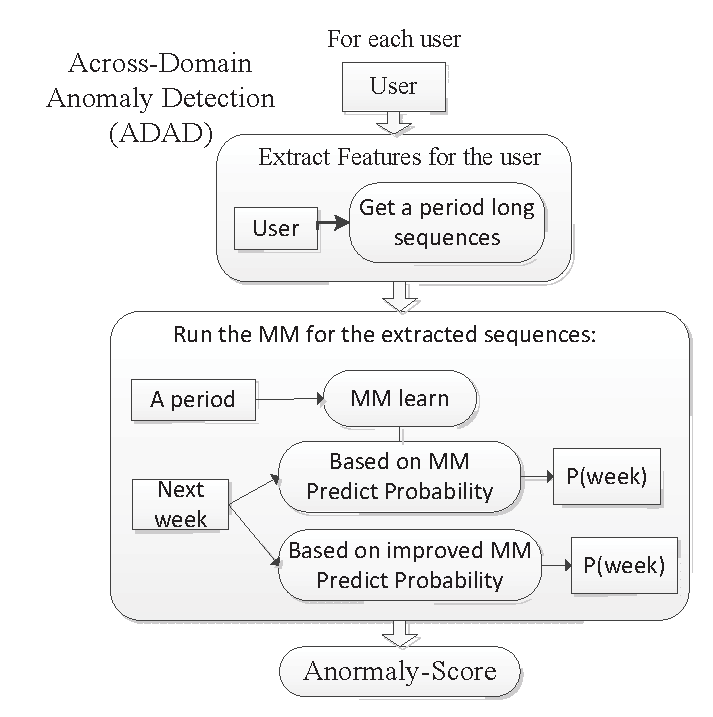
\includegraphics[width = 0.35\textwidth]{figure/figure6.eps}}
\caption{An overview of the Across-Time Anomaly Detection(ATAD).}
\label{fig}
\end{figure}
\subsubsection{Model building}
\iffalse
Feature Extraction
The CERT Dataset contains many log files which describe a particular kind of activity for all users (users being the same as employees), for instance http.csv contains logs pertaining to web browsing (website, date accessed, username, etc.). We load each file, and assign a symbol to each behavior based on the set of features we are defined in ADAD. 

For example, if a user logon between 00:00 and 06:00,we define this activity as “ALogon”, between 06:00 and 12:00,we define it as “BLogon”, between 12:00 and 18:00,we define it as “CLogon”, between 18:00 and 24:00,we define it as “DLogon”, and we treat them as different behaviors. 

After this, we join all of these files, partition them by each user and then finally sort them based on the respective timestamps. We get a list of actions and the time at which they undertook them for each user.
We then devide these actions into two parts, one is the action in a period, which gives us the final output for the feature extraction phase as the train data. The other is the next week as the test data

one is the action in last week,the other is the rest of the time, which gives us the final output for the feature extraction phase. for each part we have a sequence of actions the user took. Experimenting with the time-scale we use is an interesting avenue of research that we have not explored in this paper, but reserve for future study. 
\fi
This detection model is implemented based on Markov Models
taking historical behaviors features into account. Users have defferent behaviors on computers every day. When a user finish a behavior and begin the next behavior, a new record is created. 
The historical behaviors may be a sequence of observations \emph{$B=(a_1,a_2...,a_n)$}, in which \emph{$a_i$} is the behavior that user is served by at time \emph{t}. 

Consider a user whose behaviors history is \emph{$B = a_1a_2...a_n.$}
Let substring \emph{$B(i, j) = a_ia_{i+1}\ldots a_j$} for any \emph{$1 \textless i \textless j \textless n$}.
 We think of the user’s behaviors as a random variable \emph{X}. Let \emph{$X(i,j)$} be a string \emph{$X_iX_{i+1}\ldots X_j$} representing the sequence of random variates \emph{$X_i, X_{i+1},\ldots X_j$} for any \emph{$1\textless i \textless j \textless n$}. Define the context \emph{$c = B(n-k+1,n)$}. Let \emph{A} be the set of all possible behaviors. 
For all \emph{$a \in A $} and \emph{$i \in \{1,2,. . ., n\}$}, we let the notation \emph{$P(X_i = a_i|\ldots)$} denotes the probability that \emph{$X_i$} takes the value \emph{$a_i$}.
\iffalse
\begin{align}
	&P(X_{n+1}=a|X(1,n)=B)\notag\\
	&=P(X_{n+1}=a|X(n-k+1,n)=c)\notag\\
	&=P(X_{i+k+1}=a|X(i+1,i+k)=c),\notag
\end{align}
where the notation \emph{$P(X_i = a_i|\ldots)$} denotes the probability
that \emph{$X_i$} takes the value \emph{$a_i$}. The first two lines indicate the assumption that the probability depends only on the context of the k most recent locations. The latter two lines
indicate the assumption of a stationary distribution; that is, the probability is the same anywhere the context is the same.
\fi
These probabilities that  can be represented by a \emph{transition
probability matrix M}. Depending on the assumption of Markov, both the rows and columns of \emph{M} are
indexed by \emph{length-k} strings from \emph{$A^k$} so that
\begin{align}
	&P(X_{n+1}=a|X(1,n)=B(1,n))=M(s,s'),
\end{align}
where \emph{$s = B(n-k+1,n)$} is the current context and \emph{$s'= B(n-k+2,n)a$} is the next context. .In that case, knowing \emph{M} would immediately provide the probability for each possible next symbol of \emph{B}. In this study, we let \emph{k} equal to 0 for more historical information for building users profile.

Since we do not know \emph{M}, we can generate an estimate \emph{$\hat P$} from the current history \emph{B} using the current context \emph{c} of length \emph{k}. The probability for the next symbol to be \emph{a} is
\begin{align}
	P_k(a)=\hat P(X_{n+1}=a|B))= \frac {N(ca,B)}{N(c,B)},
\end{align}
where \emph{N(s',s)} denotes the number of times the substring \emph{s'} occurs in the string \emph{s}.

Given this estimate, we can easily define the behavior of the Markov model. It predicts the symbol \emph{$a \in A$} with the maximum probability \emph{$\hat P(X_{n+1}=a|B)$}; that is, the symbol that most frequently followed the current context \emph{c} in prior occurrences in the history. We will introduce the anomaly detection in the next section.


\subsubsection{Anomaly Detection}
In this section, an improves Markvo method(IM) proposed is to detect users' behaviors. For intrusion detection, we wanted to build a longterm norm profile of temporal behavior, and to
compare the temporal behavior in the recent past to the long-term norm profile for detecting a significant difference. Using formulae (2), we trained and built a stationary Markov chain model  of temporal behavior as the long-term norm profile by learning the transition probability matrix emph{M} from a stream of users behaviors that was observed during a period of time.

We defined the temporal behaviors in the recent past by opening up \emph{W} continuous observation windows of size \emph{N} on the continuous steam of users behaviors to view the users behaviors from the current time \emph{DN}:
\emph{$a_{11},a_{12},\dots,a_{1N},a_{21},a_{22},\dots,a_{2N},\dots,a_{DN}$}, where a stands for behavior. First, using formula (2), we compute the probability that the sequence of states \emph{$a_{11},a_{12},\dots,a_{1N},a_{21},a_{22},\dots,a_{2N},\dots,a_{DN}$} occurs in the context \emph{c} of length \emph{k}.

Second, given the \emph{M} matrix produced in the first step, the anomaly score \emph{R$_{trend}$} for the user is calculated as
\begin{align}
R_{trend}=\frac{\sum_{d=1}^D \prod_{t=1}^N P_k(a_{dn})}{D},
\end{align}
In this study, we let \emph{N} equal to a week. Because a week can build a complete profile for a user as a week cycle.

Third, after obtaining the anomaly score for all users, 
We can then set a threshold \emph{T}, which we use to classify users as anomalous or not. If the anomaly score of the user is below the threshold, we classify it as anomalous. This threshold \emph{T} is a critical parameter of our model which must be set carefully.
However, after running the improved MM Algorithm we can save the anomaly scores generated and then experiment with many values of \emph{T}. One could also imagine a human security analyst increasing T from 0 in order to be presented with more instances which the user deems anomalous.







\iffalse
In this section, an improves Markvo method(IM) proposed is to detect users' behaviors. 
We 
For insider threat detection, we propose an improved Markvo method(IM) to model behavior change. First,we need to build a period time norm profile of behavior by modeling behavior change for each user during a period of time. For every user, we computer the likelihood of transitions between behaviors and abtain a transition probability matrix \emph{A}.
Second, we compare the behavior in the recent past to
the period-time norm profile to get the anomaly score for each user and if the anomaly score exceeds a threshold we detect the user as a insider threater. 
Next, the remainder of this section is dedicated to describing the model.

First, the behavior transition probability matrix of each user is learned from the observations of the user behavior in the past. 
We extract the historical behaviors 
$B=(b_1, b_2, ..., b_n)$ and the current context $C = (c_{12},c_{13},..., c_{ij}$), $b_{ij}$ denotes that behaver $j$ happend behind behavior $i$. 
To calculate the probability of one behavior ($b_i$) transitions to the next behavior ($b_j$) and the initial probability distribution (\emph{$q_i$}) of behavior \emph{i}, 
we use a simple estimator $P_{ij}$ from the historical behaviors \emph{B} based on the assumption of Markov models\cite{b47}:
\begin{align}
P_{b_{ij}}&=N(c_{ij},C)/N(b_i,B)\\
q_{b_i}&=N({b_i},B)/N(b,B)
\end{align}
Where \emph{N($s\prime$, s)} represents the number of times the substring \emph{$s\prime$} appears in the string \emph{s}. In this way, we calculate the probability of all behaviors transition and obtain the behavior transition probability matrix for the next step.

Second, we get a new behavior sequences of the user in the next week (\emph{b$_{11}$,b$_{12}$,......b$_{DT}$}), where \emph{b$_{DT}$} denotes the behavior \emph{T} happens on the day \emph{D}. Given the \emph{A} matrix produced in the first step, the anomaly score \emph{R$_{trend}$} for the user is calculated by estimating the user’s transition likelihood over time. The anomaly probability score is computed depending on the behavior transition probability matrix caculated in the first step as
\begin{align}
R_{trend}=1/D\sum_{d=1}^D {q_{b_1}\prod_{t=2}^T P_{b_{d(t-1)}b_dt}}
\end{align}

Third, after obtaining the anomaly score for all users, 
We can then set a threshold \emph{T}, which we use to classify users as anomalous or not. If the anomaly score of the user is below the threshold, we classify it as anomalous. This threshold T is a critical parameter of our model which must be set carefully.
However, after running the improved MM Algorithm we can save the anomaly scores generated and then experiment with many values of \emph{T}. One could also imagine a human security analyst increasing T from 0 in order to be presented with more instances which the user deems anomalous.

\fi
\subsection{Information fusion}
Our goal is to combine suspicion/anomaly scores that have been generated from each of the aforementioned methods to detect anomalies.
\iffalse
We note that in a more general analytics framework, the same technique can be used to combine scores based on relative importance or surprise/risk levels.
In anomaly detection, an individual can be anomalous in one domain or at a time instance. Also, the relative suspicion of an individual can vary from one indicator (or information source) to another. However, most anomaly detection applications require a single overall conclusion about the relative suspicion of each individual.
\fi
Therefore, we developed a technique based on weight fusion to combine acorss-domain and across-time of evidence from multiple domains. In a broad sense, each source of information provides a suspicion score and the goal is to combine these scores by wight(\emph{W}) in order to identify anomalies with greater accuracy. The combined suspicion score \emph{$R_combine$} is computed as
\begin{align}
R_{combined}&= W_1*R_{ADAD}+W_2*R_{ATAD}\\
r&=\begin{cases}
\frac{W_2}{W_1}
&\mbox{if } W_1 \textgreater 0\\
1
&\mbox{if } W_1 = 0,\\
\end{cases}
\end{align}
we can then set a threshold \emph{$T_{com}$}, which we use to classify users as anomalous or not. If the suspicion score of the user is below the threshold, we classify it as anomalous.

\section{Experiment}

This section is dedicated to a comprehensive discussion of results obtained through our analysis.
In the next sections, we will introduce the performance metrics for evaluating the three detection models separately. 
We then provide a comparative assessment of our proposed models with other existing detecting insider threat methods. 


\subsection{Across-Domain Anomaly Detection(ADAD)}\label{AA}
In this section, we first introduce the performance metrics for evaluating the detection model. 
Then, in order to select domain features that have big impacts on user's behavior, we apply the principal component analysis to give a score value to each feature. 
Finally, selected domain features are evaluated by the isolation forest to detect insider threats.


\emph{1) Evaluation Metrics and Baselines:}
Because the isolation forest can give an anomaly score for each user, we consider the metrics \emph{accuracy, Precision} and \emph{recall} to quantitatively evaluate the models.  
\emph{Precision} is the
fraction of the data entries labelled malicious that are
truly malicious; \emph{recall}, also known as sensitivity or true
positive rate, is the fraction of malicious entries that are
classified correctly; \emph{accuracy} is the fraction of all entries
that are classified correctly\cite{b56}.
\iffalse
\emph{Accuracy} represents the proportion of the number of users who are detected correctly in all users by the model. \emph{Precision} represents the proportion of the number of insider threats are detected correctly in the insider threats who are detected by the model and \emph{Recall} represents the proportion of the number of insider threats are detected in all insider threats by the model.
\fi

\iffalse
\begin{align}
Accuracy&= (TP+TN)/(TP+FP+TN+FN)\\
Precision&=TP/(TP+FP)\\
Recall&=TP/(TP+FN)
\end{align}
Where \emph{TP} denotes the number of insider threaters are detected as insider threaters, \emph{TN} denotes the number of normal users are detected normal users, \emph{FP} denotes the number of insider threaters are detected normal users and \emph{FN} denotes normal users are detected insider threaters.
\fi

\emph{2) Comparative Evaluation:} Table II shows the results of running our model ADAD with different parameters.
We found that removable media domains is the most detectable (with the highest detective accuracy), while logon and file domains are harder to detect insider threats. It appears that users show great variations in their logon and file behaviors, but are more uniform in the behavior of device usages . Except that, the property of the mode is more effective than maximum to detect, which indicates that the mode represents the more significant difference between normal and abnormal. It is obvious that some features interfere with the ability to correctly identify insider threats. In particular, using the \emph{PCA} (Principal Component Analysis) to decompose of the features to a 2-D space achieves a higher predictive accuracy.


\begin{table}[tbp]
\caption{The experiment result of ADAD.}
\centering  % 表居中
\begin{tabular}{lcccc}  % {lccc} 表示各列元素对齐方式,left-l,right-r,center-c
\hline
Domian  &iForest Input &Accuracy &Precision &Recall\\ \hline
	
Logon 	& MAX &89\% &32\% &47\%\\
  & MODE &87\% &22\% &34\%\\\hline
Logoff 	& MAX &88\% &23\% &34\%\\
   & MODE &85\% &14\% &21\%\\\hline
Connet 	& MAX &78\% &65\% &27\%\\
  & MODE &79\% &70\% &28\%\\\hline
Disconnect 	& MAX &80\% &73\% &30\%\\
  & MODE &79\% &69\% &28\%\\\hline
Filecopy 	& MAX &80\% &60\% &28\%\\
  & MODE &77\% &44\% &20\%\\\hline
All properties 	& MAX &82\% &68\% &34\%\\
  & MODE &79\% &52\% &31\%\\\hline
PCA 	&PCA  &87\% &79\% &35\%\\\hline

\end{tabular}

\end{table}


\subsection{Across-Time Anomaly Detection(ATAD)}
In this section, we first introduce the performance metrics for
evaluating the detection model. We then provide a
comparative assessment of our proposed models with existing MM detection methods.

\emph{1) Evaluation Metrics and Baselines:}
We need to set a
threshold \emph{T} to classify users as anomalous or not. 
So we consider the metrics detection Receiver
Operating Characteristic curves (or \emph{ROC} curves) curve to quantitatively evaluate the models. These curves are used to plot the true-positive (correct) rate against the false-positive rate for the different possible points in a diagnostic test. In order to produce the ROC curves, we use a process of threshold varying. After obtaining the anomaly score for each user using our model, we set a value for
the threshold, check each user one-by-one, and
classify them as anomalous if \emph{score $\textgreater$ threshold}.
We then increase the threshold and repeat until no users are classified as anomalous.

\textbf{Comparison Methods.}
The improved Markov (IM)is respectively compared with existing detection Markov:

a) Markov: when caculating the anomaly score, this model regard the behavior sequences of the week as whole and treat the evaluation result of the sequences as the final anomaly score for the week.

\emph{2) Comparative Evaluation:} 
\textbf{Comparison between IM and MM.}
We apply our Across-Time Anomaly Detection(ATAD) detection result as figure6. It's obvious that the IM model is more effective than MM. For MM, if a user has once unusual change during this week, the change will has a important influence on the detection result. However, this effect can be avoided by IM. When scoring the user's behavior, IM uses the week's average anomaly score to evaluate a user's behavior, which will reduce the impact of accidental unusual change on detecting insder threats.

In other words, IM is more likely to detect abnormal changes in behavioral trends over a period of time. So it detects insider threat more robustly. 



\begin{figure}[htb]
\centerline{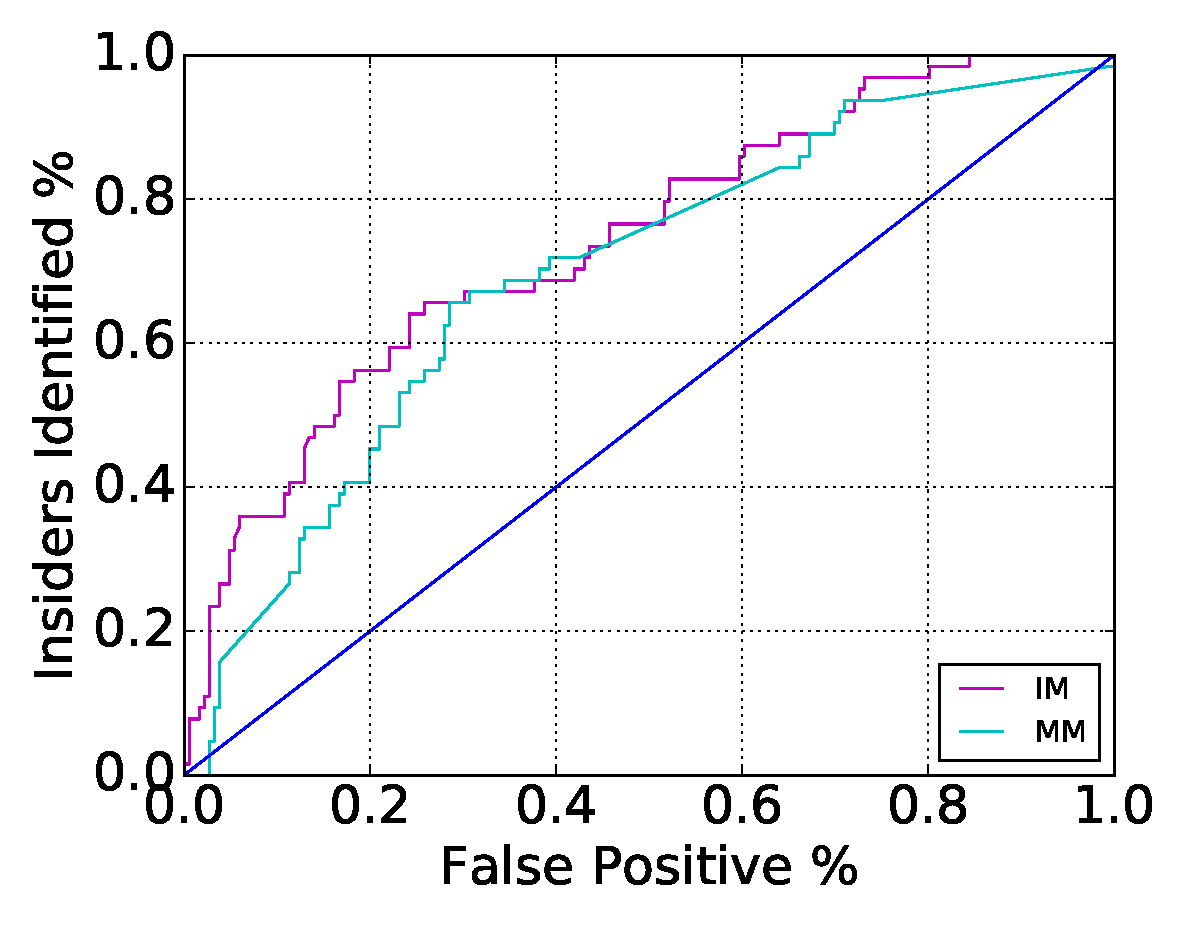
\includegraphics[width = 0.25\textwidth]{figure/figure7.eps}}
\caption{ROC Curve showing the differences between MM algorithm and improved MM algorithm.}
\label{fig}
\end{figure}


\subsection{Information fusion}
In this section,  we first introduce the performance metrics for evaluating the detection model.
we then provide a comparative assessment of our fusion method with the above two models.

\emph{1) Evaluation Metrics and Baselines:}
For the fusion method, the most important is to determine the proportion of each component. So we let \emph{r} which demotes the proportion of the two model increase from 0 to 1. Then we use the metrics \emph{accuracy, Precision} and \emph{recall} to quantitatively evaluate the models.

\emph{2) Comparative Evaluation:} 
The method based on weight fuses the ATAD and the ADAD, then get the final anomaly score. The result is shown as Table 2.
Parameter \emph{r} represents the proportion of the two methods' anomaly score. To remove amplitude variation and only focus on the underlying distribution shape on data, the scores are normalized before the weight fusion. When \emph{r} = 0, it is the result of individual ADAD method. When \emph{r} = 1, it is the result of individual ATAD method. We can see that  
only the ADAD is better than only the ATAD, and fusingh  two model is better than the ADAD. When \emph{r} values varies between 1/9 and 3/7, we can clearly see that the precision has a greater improvement. The ADAD model is based on data driven detection, and it fails to detect a malicious insider who tries to behave like a normal user to cover up his evil. However, the ATAD can make up for this deficiency by comparing behaviors of users in different time periods to detect insider threats. So, it is remarkable that a suitable combination of the individual ATAD and ADAD scores in an appropriate fashion leads to significant improvement in performance relative to any of the individual ATAD or ADAD sources. Espeicially, when \emph{r} is 3/7, the precision and recall rate is the highest, and the combination of weights is the best.

\iffalse
\begin{table}[tbp]
\caption{The experiment result of information fusion.}
\centering  % 表居中
\begin{tabular}{lcc}  % {lccc} 表示各列元素对齐方式,left-l,right-r,center-c
\hline
r  &Precision &Recall\\ \hline
0(ADAD) &79.17\% &35.19 \\\hline
1/9 &90\% &35.18\%\\\hline
2/8 &94.44\% &31.48\%\\\hline
3/7 &95\% &35.19\%\\\hline
4/6 &74.73\% &33.33\% \\\hline
5/5 &90\% &33.33\% \\\hline
6/4 &85\% &31.48\%\\\hline
7/3 &82.35\% &25.92\%\\\hline
8/2 &66.67\% &25.92\%\\\hline
9/1 &61.9\% &24.07\%\\\hline
1(ATAD) &60\% &27.78\%\\\hline
\end{tabular}

\end{table}
\fi


\begin{table*}[tbp]
\caption{The experiment result of information fusion.}
\centering  % 表居中
\begin{tabular}{lccccccccccc}  % {lccc} 表示各列元素对齐方式,left-l,right-r,center-c
\hline
r &0(ADAD)&1/9 &2/8 &3/7 &4/6 &5/5 &6/4 &7/3 &8/2 &9/1 &1(ATAD)\\\hline

Precision &79.17\% &90\% &94.44\% &\textbf{95\%}&74.73\%&90\%  &85\% &82.35\% &66.67\%&61.9\%&60\% \\\hline

Recall &35.19 &35.18\% &31.48\% &\textbf{35.19\%}&33.33\%&33.33\%&31.48\%&25.92\%&25.92\%&24.07\%&27.78\%\\\hline
\end{tabular}

\end{table*}

To get a better understanding and visualization of results based on our approach, we mark the positive sample with red and negative sample with blue. Figure 8 is an indication of how the anomaly scores are distributed when \emph{r} is 3/7 in this analysis. The graph indicated few points above the red color horizontal line which is equivalent to an anomaly score of 1.3, and the threshold is determine by \emph{ROC} curves. Users whose naomaly scores exceed the threshold can be considered as anomalous users. It reached 95\% of the accuracy. The model exists some limitations, which causes some insider threats not to be detected. 
we will present the limitation of our work in the next section.
%indicates that 95\% of the insider threaters we detected are true insider threaters.  

\begin{figure}[htb]
\centerline{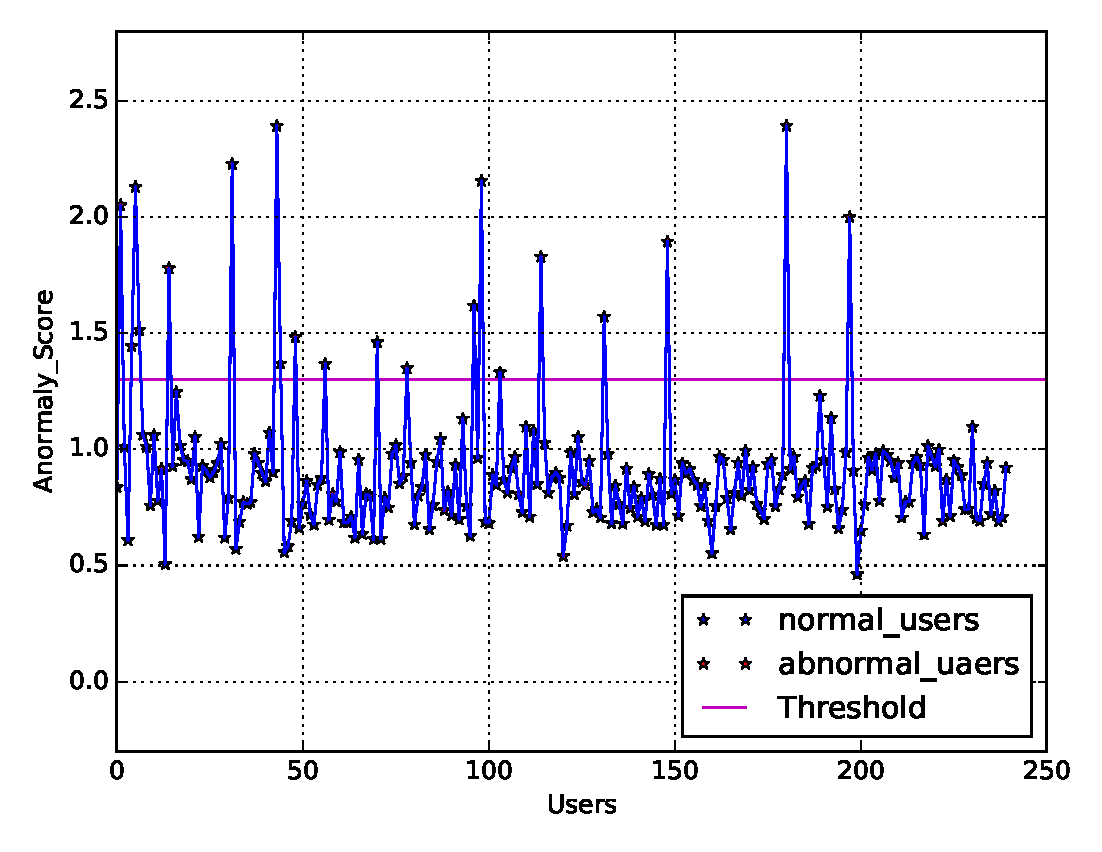
\includegraphics[width = 0.25\textwidth]{figure/figure8.eps}}
\caption{Anomaly score distribution.}
\label{fig}
\end{figure}

\section{Conclusion And Future work}

In this paper we have examined the problem of insider threat detection. We propose a hybrid model that combines a data driven model with a behavior driven model to detect insider threat in a more robust and accurate manner. 
First, the multi-dimensional features extracted from data collected  from the enterprise network is formatted and fed separately into the two separate models. Second, each model generates an abnormal score to represent the degree of users' unusual behaviors. Finally, the abnormal scores of two models are fused as the final abnormal scores for each user, and a user will be detected a insider threater if the anomaly score exceeds the threshold. After a wide range experiment, it is 
verified that the hybrid model can detect insider threats with the accuracy of 95%.



\textbf{Future work.}
We use a combined method based on weight fusion to integrate the ADAD and the ATAD, which has a high precision but a pessimistic recall. To solve this problem, we could apply on some complex and effective fusion scheme to combine their information in order to improve the recall of anomaly detection(e.g.,\cite{b49}).  In addition, we could take user role into account in generates user Normal portrait that can describe the full extent of activities that users perform within the organization based on role to improve the recall of anomaly detection(e.g.,\cite{b50}).   	

\iffalse
\section{Limitation and future work}

In the exploration into the utility of a Fusion Method based on multi-dimensional features to insider threat detection, we have made many assumptions that could limit the effectiveness of our approach in certain scenarios. We enumerate the most important of these, and the possible effect they could have on our system below.

User behavior is almost consistent in ADAD:in ADAD model, We assume that the behavior of all is basically the same, based on which we could identify people who inconsistent with the public. In fact, There are some differences in the behavior of people in different positions, it reserve for future study.

Training on a period data in ATAD: 
In order to apply our ATAD model, we must first ensure that it is able to distinguish a user’s normal behaviour from anomalous behaviour. This then means that we must train on some sample of a user’s behaviour in order for the model to learn normal behaviour. Hence we are not looking for insider threats in that training set, which in our specific case means that we do not consider that a user might attack in a period data. This could significantly hamper our ability to detect insider threats amongst short-term users (contractors for instance), which are a real threat \cite{b48}.

Features: Our approach is only able to make use of the information that it is provided, and hence depends on the features that it is supplied with. This requires domain knowledge and manual feature engineering and experimentation in order to produce useful features. Our approach would therefore need to be adapted somewhat depending on application cases.


\subsection{Future work} 
Threshold:Our current procedure for determining if the anomaly score is anomalous or not is to compare with a threshold. This requires us to manually set a threshold value, which is another hyperparameter of our system that significantly affects the results. However, we could consider the task of determining which score is anomalous as an anomaly detection problem itself. Hence, we could apply a novel outlier threshold selection algorithm that aids in analyzing the specific domain and time-instance related events that were responsible for a particular to be flagged with a high anomaly rank.(e.g., \cite{b49}) on the anomaly score generated by our model. This allows us to avoid having to manually set a threshold parameter.

Fusion method \&\& Recall \&\& Role\_based	:We use a combined method based on weight fusion to integrate the ADAD and the ATAD, which has a high precision but a pessimistic recall. To solve this problem, we could apply on some complex and effective fusion scheme to combine their information in order to improve the recall of anomaly detection(e.g.,\cite{b49}).  In addition, we could take user role into account in generates user Normal portrait that can describe the full extent of activities that users perform within the organization based on role to improve the recall of anomaly detection(e.g.,\cite{b50}).   	
\fi

\section*{Acknowledgment}

The preferred spelling of the word ``acknowledgment'' in America is without 
an ``e'' after the ``g''. Avoid the stilted expression ``one of us (R. B. 
G.) thanks $\ldots$''. Instead, try ``R. B. G. thanks$\ldots$''. Put sponsor 
acknowledgments in the unnumbered footnote on the first page.



\begin{thebibliography}{00}
\bibitem{b1}Gavai, Gaurang, et al. "Detecting Insider Threat from Enterprise Social and Online Activity Data." ACM CCS International Workshop on Managing Insider Security Threats ACM, 2015:13-20.
\bibitem{b1} Gamachchi, Anagi, L. Sun, and S. Boztas. "A Graph Based Framework for Malicious Insider Threat Detection." Hawaii International Conference on System Sciences 2017.
\bibitem{b2} Rashid, Tabish, I. Agrafiotis, and J. R. C. Nurse. "A New Take on Detecting Insider Threats: Exploring the Use of Hidden Markov Models." International Workshop 2016:47-56.
\bibitem{b3} “By the numbers: Cyber attack costs compared,” 2016, accessed on 31/05/2016. [Online]. Available: http://www.csoonline.com/article/3074826/security/bythe-numbers-cyber-attack-costs-compared.html
\bibitem{b4}  D. Cappelli, A. Moore, and R. Trzeciak, The CERT Guide to Insider Threats: How to Prevent, Detect, and Respond to Information Technology Crimes (Theft, Sabotage, Fraud). Addison-Wesley Professional, 2012
\bibitem{b5} Young, William T, et al. Use of Domain Knowledge to Detect Insider Threats in Computer Activities.  2013.
\bibitem{b6}Eldardiry H, Sricharan K, Liu J, et al. Multi-source fusion for anomaly detection: using across-domain and across-time peer-group consistency checks[J]. Computing \& Informatics, 2014, 31(3):575-606.
\bibitem{b7} Gamachchi, Anagi, L. Sun, and S. Boztas. "A Graph Based Framework for Malicious Insider Threat Detection." Hawaii International Conference on System Sciences 2017.
\bibitem{b8} Sherali   Zeadally, et al. "Detecting Insider Threats: Solutions and Trends." Information Security Journal A Global Perspective 21.4(2012):183-192.
\bibitem{b9}  D. Cappelli, A. Moore, and R. Trzeciak, The CERT Guide to Insider Threats: How to Prevent, Detect, and Respond
to Information Technology Crimes (Theft, Sabotage, Fraud). Addison-Wesley Professional, 2012
\bibitem{b10}W. L. Winston, Operations Research: Applications and Algorithms. Belmont, CA: Duxbury Press, 1994.
\bibitem{b11}  P. A. Legg et al., “Towards a conceptual model and reasoning structure for insider threat detection,” J. Wireless Mobile Netw., Ubiquitous Comput., Dependable Appl., vol. 4, no. 4, pp. 20–37, Dec. 2013.
\bibitem{b12} M. Bishop et al., “Insider threat detection by process analysis,” in Proc. IEEE SPW, 2014, pp. 251–264.
\bibitem{b13} Sunu Mathew, Michalis Petropoulos, Hung Q Ngo, and Shambhu Upadhyaya. A data-centric approach to insider attack detection in database systems. In Recent Advances in Intrusion Detection, pages 382–401. Springer, 2010.
\bibitem{b14} William Eberle, Jeffrey Graves, and Lawrence Holder. Insider threat detection using a graph-based approach. Journal of Applied Security Research, 6(1):32–81, 2010.
\bibitem{b15} H. Eldardiry et al., “Multi-domain information fusion for insider threat detection,” in Proc. IEEE SPW, May 2013, pp. 45–51.
\bibitem{b16}Automated Insider Threat Detection System Using User and Role-Based Profile Assessment Philip A. Legg, Oliver Buckley, Michael Goldsmith, and Sadie Creese


\iffalse
\bibitem{b1}A. M. Dawn Cappelli Randall Trzeciak,Timothy J. Shimeall,“Common Sense Guide to Prevention and Detection of Insider
Threats , 3rd Edition,” 2009.
\bibitem{b2} Gemalto. Breach level index|data breach database \& risk assessment calculator, 2016. http://www.breachlevelindex.com/.
\bibitem{b3} “By the numbers: Cyber attack costs compared,” 2016, accessed on 31/05/2016. [Online]. Available: http://www.csoonline.com/article/3074826/security/bythe-numbers-cyber-attack-costs-compared.html
\bibitem{b4} Teresa F Lunt. A survey of intrusion detection techniques. Computers \& Security, 12(4):405–418, 1993.
\bibitem{b5} Sunu Mathew, Michalis Petropoulos, Hung Q Ngo, and Shambhu Upadhyaya. A data-centric approach to insider attack detection in database systems. In Recent Advances in Intrusion Detection, pages 382–401. Springer, 2010.
\bibitem{b6} William Eberle, Jeffrey Graves, and Lawrence Holder. Insider threat detection using a graph-based approach. Journal of Applied Security Research, 6(1):32–81, 2010.
\bibitem{b7} Alex Memory, Henry G Goldberg, and E Ted. Context-aware insider threat detection. In Workshops at the Twenty-Seventh AAAI Conference on Artificial
Intelligence, 2013.
\bibitem{b8} Robert F Mills, Michael R Grimaila, Gilbert L Peterson, and Jonathan W Butts. A scenario-based approach to mitigating the insider threat. Technical report, DTIC Document, 2011.
\bibitem{b9}  D. Cappelli, A. Moore, and R. Trzeciak, The CERT Guide to Insider Threats: How to Prevent, Detect, and Respond
to Information Technology Crimes (Theft, Sabotage, Fraud). Addison-Wesley Professional, 2012
\bibitem{b10}  Miltiadis Kandias, Alexios Mylonas, Nikos Virvilis, Marianthi Theoharidou, and Dimitris Gritzalis. An insider threat prediction model. In Trust, privacy and security in digital business, pages 26–37. Springer, 2010.
\bibitem{b11}Frank L Greitzer, Lars J Kangas, Christine F Noonan,and Angela C Dalton. Identifying at-risk employees: A behavioral model for predicting potential insider threats. Pacific Northwest National Laboratory Richland, WA, 2010
\bibitem{b12}GB Magklaras and SM Furnell. Insider threat prediction tool: Evaluating the probability of it misuse. Computers \& Security, 21(1):62–73, 2001.
\bibitem{b13}Hoda Eldardiry, Evgeniy Bart, Juan Liu, John Hanley, Bob Price, and Oliver Brdiczka. Multi-domain information fusion for insider threat detection. In Security and Privacy Workshops (SPW), 2013 IEEE, pages 45–51. IEEE, 2013.
\bibitem{b14}Automated Insider Threat Detection System Using User and Role-Based Profile Assessment Philip A. Legg, Oliver Buckley, Michael Goldsmith, and Sadie Creese
\bibitem{b15}  Deep Learning for Unsupervised Insider Threat Detection in Structured Cybersecurity Data Streams Aaron Tuor and Samuel Kaplan and Brian Hutchinson∗
Western Washington University Bellingham, WA Nicole Nichols and Sean Robinson Pacific Northwest National Laboratory Seattle, WA
\bibitem{b16}  P. A. Legg et al., “Towards a conceptual model and reasoning structure for insider threat detection,” J. Wireless Mobile Netw., Ubiquitous Comput., Dependable Appl., vol. 4, no. 4, pp. 20–37, Dec. 2013.
\bibitem{b17} M. Bishop et al., “Insider threat detection by process analysis,” in Proc. IEEE SPW, 2014, pp. 251–264.
\bibitem{b18}] M. Bishop, S. Engle, S. Peisert, S. Whalen, and C. Gates, “We have met the enemy and he is us,” in Proc. NSPW, Lake Tahoe, CA, USA, Sep. 2008, pp. 1–12
\bibitem{b19} J. R. C. Nurse et al., “Understanding insider threat: A framework for characterising attacks,” in Proc. IEEE SPW, 2014, pp. 214–228
\bibitem{b20}F. Kammueller and C. W. Probst, “Invalidating policies using structural information,” J. Wireless Mobile Netw., Ubiquitous Comput., Dependable Appl., vol. 5, no. 2, pp. 59–79, Jun. 2014.
\bibitem{b21} M. R. Ogiela and U. Ogiela, “Linguistic protocols for secure information management and sharing,” Comput. Math. Appl., vol. 63, no. 2, pp. 564–572, Jan. 2012.
\bibitem{b22}G. B. Magklaras and S. M. Furnell, “Insider threat prediction tool: Evaluating the probability of IT misuse,” Comput. Security, vol. 21, no. 1, pp. 62–73, 1st Quart. 2002.
\bibitem{b23} L. Spitzner, “Honeypots: Catching the insider threat,” in Proc. 19th IEEE ACSAC, Las Vegas, NV, USA, Dec. 2003, pp. 170–179.
\bibitem{b24}G. B. Magklaras and S. M. Furnell, “Insider threat prediction tool: Evaluating the probability of IT misuse,” Comput. Security, vol. 21, no. 1, pp. 62–73, 1st Quart. 2002.
\bibitem{b25} J. Myers, M. R. Grimaila, and R. F. Mills, “Towards insider threat detection using web server logs,” in Proc. 5th Annu. CSIIRW—Cyber Security Inf. Intell. Challenges Strategies, New York, NY, USA, 2009, pp. 54:1–54:4.
\bibitem{b26} M. A. Maloof and G. D. Stephens, “Elicit: A system for detecting insiders who violate need-to-know,” in Recent Advances in Intrusion Detection, vol. 4637, Lecture Notes in Computer Science, C. Kruegel, R. Lippmann, and A. Clark, Eds. Berlin, Germany: Springer-Verlag, 2007, pp. 146–166.
\bibitem{b27} J. S. Okolica, G. L. Peterson, and R. F. Mills, “Using PLSI-U to detect insider threats by datamining e-mail,” Int. J. Security Netw., vol. 3, no. 2, pp. 114–121, 2008.
\bibitem{b28}Y. Liu et al., “SIDD: A framework for detecting sensitive data exfiltration sby an insider attack,” in Proc. 42nd HICSS, Jan. 2009, pp. 1–10.
\bibitem{b29} H. Eldardiry et al., “Multi-domain information fusion for insider threat detection,” in Proc. IEEE SPW, May 2013, pp. 45–51.
\bibitem{b30} Brdiczka et al., “Proactive insider threat detection through graph learning and psychological context,” in Proc. IEEE Symp. SPW, San Francisco, CA, USA, May 2012, pp. 142–149.
\bibitem{b31}W. Eberle, J. Graves, and L. Holder, “Insider threat detection using a graph-based approach,” J. Appl. Security Res., vol. 6, no. 1, pp. 32–81, Dec. 2010.
\bibitem{b32}B. Klimt and Y. Yang, “The enron corpus: A new dataset for email classification research,” in Machine Learning: ECML 2004, vol. 3201, Lecture Notes in Computer Science, J.-F. Boulicaut, F. Esposito, F. Giannotti, and D. Pedreschi, Eds. Berlin, Germany: Springer-Verlag, 2004, pp. 217–226
\bibitem{b33}T. E. Senator et al., “Detecting insider threats in a real corporate database of computer usage activity,” in Proc. 19th ACM SIGKDD Int. Conf. Knowl. Discov. Data Mining, 2013, pp. 1393–1401.
\bibitem{b34}P. Parveen, J. Evans, B. Thuraisingham, K. W. Hamlen, and L. Khan, “Insider threat detection using stream mining and graph mining,” in Proc. IEEE 3rd Int. Conf. Social Comput. PASSAT, Oct. 2011, pp. 1102–1110.
\bibitem{b35}P. Parveen and B. Thuraisingham, “Unsupervised incremental sequence learning for insider threat detection,” in Proc. IEEE Int. Conf. ISI, Jun. 2012, pp. 141–143.
\bibitem{b36}S. Greenberg, Using unix: Collected traces of 168 users, Univ. Calgary, Calgary, AB, Canada, Tech. Rep., 1988.
\bibitem{b37} Rashid, Tabish, I. Agrafiotis, and J. R. C. Nurse. "A New Take on Detecting Insider Threats: Exploring the Use of Hidden Markov Models." International Workshop 2016:47-56.
\bibitem{b38}Automated Insider Threat Detection System Using User and Role-Based Profile Assessment Philip A. Legg, Oliver Buckley, Michael Goldsmith, and Sadie Creese
\bibitem{b39}“CERT Insider Threat Data Set,” Software Engineering Institute, Carnegie Mellon University, CERT Division and Exact
Data LLC. [Online]. Available: https://www.cert.org/insiderthreat/tools/
\bibitem{b40}D. Cappelli, A. Moore, and R. Trzeciak, The CERT Guide to Insider Threats: How to Prevent, Detect, and Respond
to Information Technology Crimes (Theft, Sabotage, Fraud). Addison-Wesley Professional, 2012.
\bibitem{b41} D. Cappelli, A. Moore, and R. Trzeciak, The CERT Guide to Insider Threats: How to Prevent, Detect, and Respond
to Information Technology Crimes (Theft, Sabotage, Fraud). Addison-Wesley Professional, 2012.
\bibitem{b42}I. Jolliffe, Principal Component Analysis. Hoboken, NJ, USA: Wiley,2005.
\bibitem{b43}F. T. Liu, K. M. Ting, and Z. H. Zhou, “Isolation forest,” in 2008 Eighth IEEE International Conference on Data Mining,
Dec 2008, pp. 413–422
\bibitem{b44}L. Sun, S. Versteeg, S. Boztas, and A. Rao, “Detecting anomalous user behaviour using an extended Isolation Forest algorithm: An enterprise case study,” Sept 2016, arXiv:1609.06676.
\bibitem{b45}W. L. Winston, Operations Research: Applications and Algorithms. Belmont, CA: Duxbury Press, 1994.
\bibitem{b46}W. L. Winston, Operations Research: Applications and Algorithms. Belmont, CA: Duxbury Press, 1994.
\bibitem{b47}T. M. Mitchell, Machine Learning. Boston,
MA: McGraw-Hill, 1997.
\bibitem{b48} J. R. C. Nurse, O. Buckley, P. A. Legg, M. Goldsmith, S. Creese, G. R. Wright, and M. Whitty. Understanding insider threat: A framework for characterising attacks. In IEEE Security and Privacy Workshops (SPW). IEEE, 2014. DOI: 10.1109/SPW.2014.38.
\bibitem{b49}Eldardiry H, Sricharan K, Liu J, et al. Multi-source fusion for anomaly detection: using across-domain and across-time peer-group consistency checks[J]. Computing \& Informatics, 2014, 31(3):575-606.
\bibitem{b50} Legg P A, Buckley O, Goldsmith M, et al. Automated Insider Threat Detection System Using User and Role-Based Profile Assessment[J]. IEEE Systems Journal, 2017, 11(2):503-512.
\bibitem{b51} Young, William T, et al. Use of Domain Knowledge to Detect Insider Threats in Computer Activities.  2013.
\bibitem{b52} Gamachchi, Anagi, L. Sun, and S. Boztas. "A Graph Based Framework for Malicious Insider Threat Detection." Hawaii International Conference on System Sciences 2017.

\bibitem{b53} Sherali   Zeadally, et al. "Detecting Insider Threats: Solutions and Trends." Information Security Journal A Global Perspective 21.4(2012):183-192.

\bibitem{b54} Ye, Nong. "A Markov Chain Model of Temporal Behavior for Anomaly Detection." 2000:171--174.
\bibitem{b55} Lv, Qiujian, et al. "Big Data Driven Hidden Markov Model Based Individual Mobility Prediction at Points of Interest." IEEE Transactions on Vehicular Technology PP.99(2016):1-1.

\bibitem{b56} Li, Ling Ko, et al. "Insider threat detection and its future directions." International Journal of Security & Networks 12.3(2017):168.

\fi








\end{thebibliography}

\end{document}
